\documentclass[11pt]{article}

% load some asm stuff -
\usepackage{amssymb}
\usepackage{amsmath}
\usepackage{amsthm}
%\usepackage{palatino,lettrine}
\usepackage{fancyhdr}
\usepackage{epsfig}
\usepackage[square,sort,comma,numbers]{natbib}
\usepackage{simplemargins}
\usepackage{setspace}
\usepackage{wrapfig}
\usepackage{hyperref}
%\usepackage{boiboites}
\usepackage[margin=0pt,font=small,labelfont=bf]{caption}
\newcommand{\boldindex}[1]{\textbf{\hyperpage{#1}}}
\usepackage{makeidx}\makeindex
\bibliographystyle{plos2015}

\usepackage{algpseudocode}
\usepackage{algorithm}


% Set the size
%\textwidth = 6.75 in
%\textheight = 9.75 in
%\oddsidemargin = 0.0 in
%\evensidemargin = 0.0 in
%\topmargin = 0.01 in
%\headheight = 0.0 in
%\headsep = 0.25 in
%\parskip = 0.15in
% \doublespace
\setallmargins{1in}

\newtheorem{example}{Example}[section]
\newtheorem{thm}{Theorem}[section]
\newtheorem{property}{Property}[section]

\theoremstyle{definition}
\newtheorem{defn}[thm]{Definition}

\makeatletter
% \renewcommand\subsection{\@startsection
% 	{subsection}{2}{0mm}
% 	{-0.05in}
% 	{0.05\baselineskip}
% 	{\normalfont\normalsize\bfseries}}
\renewcommand\subsubsection{\@startsection
	{subsubsection}{2}{0mm}
	{-0.05in}
	{-0.5\baselineskip}
	{\normalfont\normalsize\itshape\bfseries}}
\renewcommand\paragraph{\@startsection
	{paragraph}{2}{0mm}
	{-0.05in}
	{-0.5\baselineskip}
	{\normalfont\normalsize\itshape}}
\makeatother
\linespread{1.1}

\fancypagestyle{proposal}{\fancyhf{}%
	\fancyhead[RO,LE]{\thepage}%
	\fancyhead[LO,RE]{CHEME 132 Module 1 Binomial Models of Equity Prices}%
	\renewcommand\headrulewidth{1pt}}
\pagestyle{proposal}

\usepackage{mdframed}
\definecolor{lgray}{rgb}{0.92,0.92,0.92}
\definecolor{antiquewhite}{rgb}{0.98,0.92,0.84}
\definecolor{lightskyblue}{rgb}{0.93,0.95,0.99}

% defn environment
\mdfdefinestyle{theoremstyle}{% 
    linecolor=black,linewidth=1pt,% 
    frametitlerule=true,% 
    frametitlebackgroundcolor=lgray, 
    innertopmargin=\topskip,} 
\mdtheorem[style=theoremstyle]{definition}{Definition}

% concept environment
\mdfdefinestyle{conceptstyle}{% 
    linecolor=black,linewidth=1pt,% 
    frametitlerule=true,% 
    frametitlebackgroundcolor=lightskyblue, 
    innertopmargin=\topskip,} 
\mdtheorem[style=conceptstyle]{concept}{Concept}
\newcommand{\newterm}[1]{{\it #1}}

% Single space'd bib -
\setlength\bibsep{0pt}

\renewcommand{\rmdefault}{phv}\renewcommand{\sfdefault}{phv}
%\newboxedtheorem[boxcolor=black, background=gray!5,titlebackground=orange!20,titleboxcolor = black]{color_box_example}{Example}{test}

% Change the number format in the ref list -
\renewcommand{\bibnumfmt}[1]{#1.}

% Change Figure to Fig.
\renewcommand{\figurename}{Fig.}
\usepackage{enumitem}
\setlist{noitemsep} % or \setlist{noitemsep} to leave space around whole list

%Joycelyn Chan, Joshua Lequieu, Michael Paull, Chidanand Balaji, Ryan Tasseff
%Our derivation follows closely the earlier development of Fredrickson \citep{Fredrickson:1976fk}.

% Begin ...
\begin{document}

%\begin{titlepage}
{\par\centering\textbf{\Large CHEME 132 Module 1: Lattice Models of Equity Share Price}}
\vspace{0.2in}
{\par \centering \large{Jeffrey D. Varner}}
\vspace{0.05in}
{\par \centering \large{Smith School of Chemical and Biomolecular Engineering}}
{\par \centering \large{Cornell University, Ithaca NY 14853}}
% \vspace{0.1in}
% {\par \centering \small{Copyright \copyright\ Jeffrey Varner 2018. All Rights Reserved.}}\\

%\end{titlepage}
\date{}
\thispagestyle{empty}

\setcounter{page}{1}

\section*{Introduction}
A lattice model discretizes the potential future states of the world into a finite number of options. 
For instance, a binomial lattice model has two future states: \texttt{up} and \texttt{down}, while a ternary lattice model has three: \texttt{up}, \texttt{down}, and \texttt{flat}. 
To make predictions, we must assign values and probabilities to each of these future states and then calculate the expected value and variance of future values. 
Thus, we do not precisely know quantities such as share price because we are projecting into the future. Instead, we have only a probabilistic model of the possible future values. 
We'll begin with the simplest possible lattice model, a binomial lattice (Fig. \ref{fig:binomial-lattice-schematic}).
\begin{figure}[h]
    \centering
    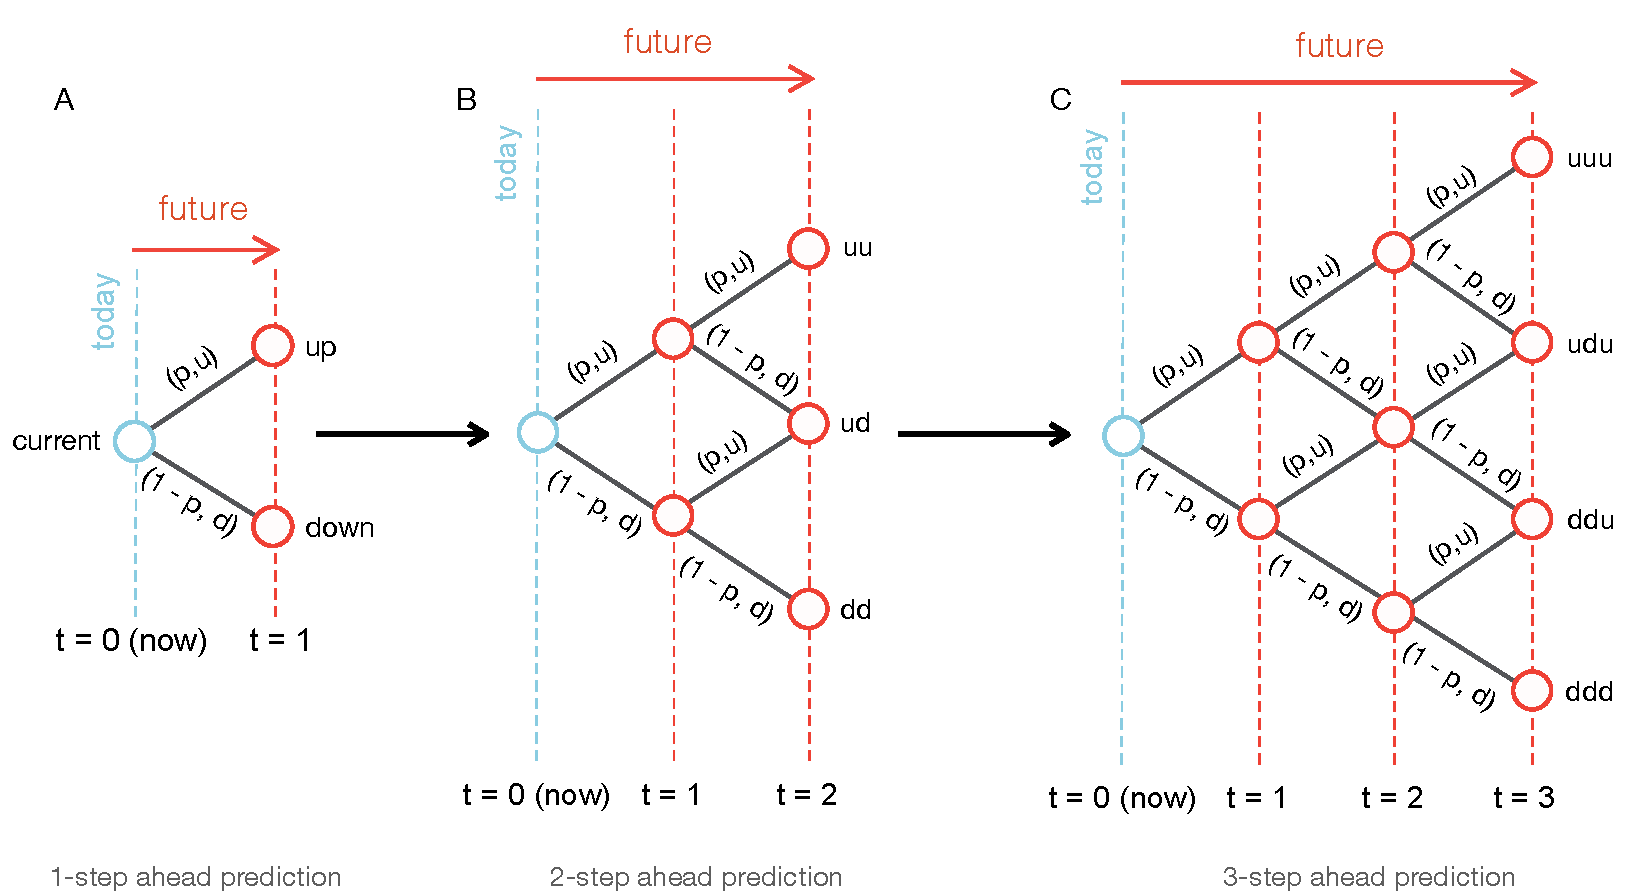
\includegraphics[width=0.85\textwidth]{./figs/Fig-Binomial-LatticeModels-Schematic.pdf}
    \caption{Binomial lattice model schematic. 
	At each node, the share price can either go \texttt{up} by $u$ or \texttt{down} by $d$. 
	The probability of going \texttt{up} is $p$, and the probability of going \texttt{down} is $1-p$. 
	\textbf{A}: Single time-step lookahead.
	\textbf{B}: Two time-step lookahead.
	\textbf{C}: Three time-step lookahead.
	At level of the tree $l$, the potential share price can take on $l+1$ values.
	}\label{fig:binomial-lattice-schematic}
\end{figure}

Let's start with a single time-step lookahead, with two possible future states (Fig. \ref{fig:binomial-lattice-schematic}A).
Let the initial share price at time \texttt{0} be $S_{\circ}$ and the share price at future time \texttt{1} be $S_{1}$.
During the transition from time \texttt{0}$\rightarrow$\texttt{1}, the world transitions from the current state to one of two possible future states: \texttt{up} or \texttt{down}.
We move to the \texttt{up} state with probability $p$ or the \texttt{down} state with probability $(1-p)$.
Thus, at the time \texttt{1}, the share price $S_{1}$ can take on one of two possible values: $S^{u} = u\cdot{S_{\circ}}$ if the world moves 
to the \texttt{up} state, or $S^{d} = d\cdot{S_{\circ}}$ if the world moves to the \texttt{down} state. 
As we move to the future, we can continue to build out the lattice model by adding additional time steps; for example, consider a two-step ahead prediction (Fig. \ref{fig:binomial-lattice-schematic}B). 
At time \texttt{2}, the share price can take on one of three possible values: $S^{uu} = u^{2}\cdot{S_{\circ}}$ if the world moves
to the \texttt{up-up} state, $S^{ud} = ud\cdot{S_{\circ}}$ if the world moves to the \texttt{up-down} state, or $S^{dd} = d^{2}\cdot{S_{\circ}}$ if the world moves to the \texttt{down-down} state.
We can continue to build out the lattice model by adding additional time steps; for example, consider a three-step ahead prediction (Fig. \ref{fig:binomial-lattice-schematic}C).

\section*{Analytical solution}
Let's consider a binomial lattice model with $n$ time-steps. At each time step, the share price can either go \texttt{up} by a factor of $u$ or \texttt{down} by a factor of $d$.
Then, at time \texttt{n}, the share price can take on $n+1$ possible values: 
\begin{equation}
	S_{n} = S_{\circ}\times{D_{1}}\times{D_{2}}\times{D_{3}}\times\cdots\times{D_{n}}
\end{equation}
where $D_{i}$ is a random variable that can take on one of two values: $u$ or $d$, 
with probabilities $p$ and $(1-p)$ respectively. 
Thus, at each time-step, the world flips a coin and lands in either the \texttt{up} state with probability $p$ or the \texttt{down} state with probability $(1-p)$.
For a single time step, we model this random process as a Bernoulli trial, where the probability of success is $p$ and the probability of failure is $(1-p)$.
As the number of time steps increases, we have a series of Bernoulli trials, which is a binomial distribution (Defn: \ref{defn-binomial-distribution}):

\begin{definition}[Binomial Share Price and Probability]\label{defn-binomial-distribution}
	Let $S_{\circ}$ denote the current share price at t = \texttt{0}, $u$ and $d$ denote the \texttt{up} and \texttt{down} factors, 
	and $p$ denote the probability of going \texttt{up}.
	At time $t$, the binomial lattice model predicts the share price $S_{t}$ is given by:
	\begin{equation*}
	S_{t} = S_{\circ}\cdot{u}^{t-k}\cdot{d}^{k}\qquad\text{for}\quad{k=0,1,\dots,t}
	\end{equation*}
	The probability that the share price takes on a particular value at time $t$ is given by:
	\begin{equation*}
	P(S_{t} = S_{\circ}\cdot{u}^{t-k}\cdot{d}^{k}) = \binom{t}{k}\cdot{(1-p)}^{k}\cdot{p}^{t-k}\qquad\text{for}\quad{k=0,1,\dots,t}
	\end{equation*}
	where $\binom{t}{k}$ denotes the binomial coefficient.
\end{definition}

\section*{Models of $u$, $d$ and $p$}
The \texttt{up} and \texttt{down} factors $u$ and $d$, and the probability $p$ can be computed in various ways.  
For example, we can estimate them from historical data or propose models for their values. 
Let's start by looking at approaches to estimate these parameters from historical data,
and then we'll introduce an imprtant model developed by Cox, Ross and Rubinstein (CRR) to compute $u$, $d$ and $p$ in the 
context of options pricing that we'll see later \citep{COX1979229}.

\subsection*{Real-world probability $p$}
Suppose we have a historical share price dataset from time $1,\dots, T$ for some ticker $j$ denoted as $\mathcal{D}_{j} = \left\{S^{(j)}_{1},S^{(j)}_{2},\dots, S^{(j)}_{T}\right\}$, 
where $S^{(j)}_{i}$ denotes the share price of ticker $j$ at time $i$.
We can use different values for the share price, e.g., the opening price, closing price, high price, low price, etc. 
In our case, when dealing with historical data, we will typically use the volume-weighted average price (VWAP) for the period, 
e.g., the VWAP for the day, week, month, etc. Over the time range of the dataset $\mathcal{D}_{j}$, we can calculate the number of \texttt{up} and \texttt{down} moves
occurring between time $i-1$ and $i$, and the magnitude of these moves. 
Then, the fraction of \texttt{up} moves is an estimate of the probability $p$, 
while some measured of the magnitude of the \texttt{up} and \texttt{down} moves, e.g., the average value are estimates of $u$ and $d$ respectively.

Suppose we assume the share price of ticker $j$ is continuously compounded with an instantaneous discount (interest) rate of 
$r^{(j)}_{i,i-1}\equiv\mu^{(j)}_{i,i-1}\cdot\Delta{t}$, i.e., we split the return into a growth rate $\mu^{(j)}_{i,i-1}$ and a time step size $\Delta{t}$.
Then, the share price at time an expression of the form governs $i$:
\begin{equation}\label{eqn:share-price-growth-rate}
S^{(j)}_{i} = \exp\left(\mu_{i,i-1}\cdot\Delta{t}\right)\cdot{S^{(i)}_{i-1}}
\end{equation}
where $\mu^{(j)}_{i,i-1}$ denotes the \textit{growth rate} (units: 1/time) for ticker $j$, and $\Delta{t}$ (units: time) 
is the time step size during the time period $(i-1)\rightarrow{i}$.
Solving for the growth rate (and dropping the ticker $j$ superscript for simplicity) gives:
\begin{equation}
\mu_{i,i-1} = \left(\frac{1}{\Delta{t}}\right)\cdot\ln\left(\frac{S_{i}}{S_{i-1}}\right)
\end{equation}
We'll often use daily price data; thus, a single trading day is a natural time frame between $S_{i-1}$ and $S_{i}$. 
However, subsequently, it will be easier to use an annualized value for the $\mu$ parameter; thus, we let $\Delta{t} = 1/252$, 
i.e., the fraction of an average trading year that occurs in a single trading day; thus, our base time will be years.
We compute the growth rate for each trading day $i$ in a collection of datasets $\mathcal{D}$ using Algorithm \ref{algo-log-return-distributions-equity}.
\begin{algorithm}[h]
    \caption{Logarithmic excess growth rate}\label{algo-log-return-distributions-equity}
    \begin{algorithmic}[1]
        
        \Require Collection of price datasets $\mathcal{D}$, where $\mathcal{D}_{j}\in\mathcal{D}$. All datasets have the same length $N$.	
		\Require list of stocks $\mathcal{L}$, where $\dim\mathcal{L} = M$.
        \Require time step size $\Delta{t}$ between $t$ and $t-1$ (units: years), 
        \Require risk-free rate $r_{f}$ (units: inverse years).

		\Statex
		\State{$M\leftarrow\text{length}(\mathcal{D}_{1})$}\Comment{Number of trading days in the dataset $\mathcal{D}_{j}$}
		\State{$N\leftarrow\text{length}(\mathcal{L})$}\Comment{Number of stocks in the dataset $\mathcal{D}$}
		\State{$\mu\leftarrow\text{Array}(M-1,N)$}\Comment{Initialize empty array of growth rates}
     
        \Statex
        \For{$i\in\mathcal{L}$}
			\State{$\mathcal{D}_{i} \gets \mathcal{D}[i]$}\Comment{Get dataset for stock $i$}

            \For{$t=2\rightarrow{N}$}
				\State{$S_{1} \gets \text{VWAP}(\mathcal{D}_{i}[t-1])$}\Comment{Get volume weighted average price for stock $i$ at time $t-1$}
				\State{$S_{2} \gets \text{VWAP}(\mathcal{D}_{i}[t])$}\Comment{Get volume weighted average price for stock $i$ at time $t$}
                
				\State{$\mu[t-1,i] \gets \left(\frac{1}{\Delta{t}}\right)\cdot\ln\left(\frac{S_{2}}{S_{1}}\right) - r_{f}$}\Comment{Set $r_{f} = 0$ for regular growth rate}
            \EndFor
        \EndFor
	
    \end{algorithmic}
\end{algorithm}
Then we can estimate the \texttt{up} and \texttt{down} factors $u$ and $d$ from the growth rate array 
generated using something like Algorithm \ref{algo-ud-estimation-equity}. 
\begin{algorithm}[h]
	\caption{Estimating $u$, $d$ and $p$ from the $\mu$-array}\label{algo-ud-estimation-equity}
	\begin{algorithmic}[1]

		\Require $\mu$-array from Algorithm \ref{algo-log-return-distributions-equity}.

		\Statex
		\State{$\mu\leftarrow\text{sort}(\mu_{i,i-1})$}
		\State{$N\leftarrow\text{length}(\mu)$}\Comment{Number of growth rates}
		
		\Statex
   	 	\State{$i_{+}\leftarrow \text{findall}(\mu>0)$}\Comment{Find the indices of all \texttt{positive} growth rates}
    	\For{$i\in {i_{+}}$}
        	\State{$\mu[i]\rightarrow(\mu\rightarrow\text{push!}(\text{up}, \exp(\mu\cdot{\Delta{t}})))$}\Comment{Push the \texttt{positive} return $\mu\cdot\Delta{t}$ onto $\text{up}$-array}
    	\EndFor
		\State{$u\leftarrow\text{mean}(\texttt{up})$}\Comment{mean is our estimate of the \texttt{up} factor $u$}
    	
		\Statex
   	 	\State{$i_{-}\leftarrow \text{findall}(\mu<0)$}\Comment{Find the indices of all \texttt{negative} growth rates}
    	\For{$i\in {i_{i}}$}
        	\State{$\mu[i]\rightarrow(\mu\rightarrow\text{push!}(\text{down}, \exp(\mu\cdot{\Delta{t}})))$}\Comment{Push the \texttt{negative} return $\mu\cdot\Delta{t}$ onto $\text{down}$-array}
    	\EndFor
		\State{$d\leftarrow\text{mean}(\texttt{down})$}\Comment{mean is our estimate of the \texttt{down} factor $d$}

		\Statex
		\State{$N_{+} \leftarrow\text{length}(i_{+})$}\Comment{Number of \texttt{positive} growth rates}
		\State{$p\leftarrow N_{+}/N$}\Comment{Estimate of the probability $p$}

		\Statex
		\Return{$u$, $d$ and $p$}
	\end{algorithmic}
\end{algorithm}
While this strategy is simple, it may not be robust. For example, if the dataset $\mathcal{D}_{j}$ is short, i.e., only a few trading days,
then the number of \texttt{up} and \texttt{down} moves will be small, and the estimates of $u$, $d$ and $p$ will be poor.
If a precise estimate of $u$, $d$ and $p$ is required, the number of trading days in the dataset $\mathcal{D}_{j}$ should be large.
Furthermore, the estimates of $u$, $d$ and $p$ are not robust to outliers in the dataset $\mathcal{D}_{j}$.
Thus, we may want to consider other models for computing $u$, $d$ and $p$.

\subsection*{Risk-neutral probability $q$}
Another approach to computing the parameters in the lattrice is to use the risk-neutral probability $q$. 
Let's consider a single-step binomial lattice model (Fig. \ref{fig:binomial-lattice-schematic}A). 
The  expected value of the share price at time \texttt{1} for a single step is given by:
\begin{equation*}
	\mathbb{E}_{\mathbb{Q}}(S_{1} | S_{\circ}) = q\cdot{S^{u}} + (1-q)\cdot{S^{d}}
\end{equation*}
where $\mathbb{E}_{\mathbb{Q}}(\dots)$ denotes the expectation operator written with respect to the risk-neutral probability measure $\mathbb{Q}$, 
the term $q$ denotes the risk-neutral probability of the \texttt{up} state, and $S^{u}$ and $S^{d}$ are the share prices in the \texttt{up} and \texttt{down} states respectively.
The hypothetical probability $q$ is used to price derivatives (as we shall see later), 
however, we could also think of it as a tool to compute a \textit{fair} price for a share of stock.
Suppose we rewrite Eqn. \eqref{eqn:share-price-growth-rate} as:
\begin{equation}\label{eqn:share-price-growth-rate-2}
    \mathcal{D}_{1,0}(\bar{r})\cdot{S_{\circ}} = \mathbb{E}_{\mathbb{Q}}\left(S_{1}|S_{\circ}\right)
\end{equation}
where $\mathcal{D}_{1,0}(\bar{r})$ is the continuous discount factor between period $0\rightarrow{1}$, 
and $\bar{r}$ is the effective (constant) risk-free rate. Thus, unlike the previous case, where the share price $S_{i}$ was discounted by the
return $\mu_{i,i-1}\cdot\Delta{t}$ (which could vary in time), here we discount the share price $S_{i}$ by an effective (constant) risk-free rate $\bar{r}$.
The expectation operator $\mathbb{E}_{\mathbb{Q}}(\dots)$ can be matched with the expansion:
\begin{equation}\label{eqn:expectation-operator-risk-neutral}
\mathcal{D}_{1,0}(\bar{r})\cdot{S_{\circ}} = q\cdot{S^{u}} + (1-q)\cdot{S^{d}}
\end{equation}
The share prices in the \texttt{up} and \texttt{down} states are the product of the \texttt{up} factor $u$ (or a \texttt{down} factor $d$) and the initial share price, 
i.e., $S^{u} = u\cdot{S_{\circ}}$ and $S^{d} = d\cdot{S_{\circ}}$. Substiuting these price values into Eqn. \eqref{eqn:expectation-operator-risk-neutral} and solving for $q$ gives:
\begin{equation}\label{eqn:risk-neutral-probability}
q = \frac{\mathcal{D}_{1,0}(\bar{r}) - d}{u - d}
\end{equation}
Thus, we can compute the risk-neutral probability $q$ from the \texttt{up} and \texttt{down} factors $u$ and $d$ 
and the effective risk-free rate $\bar{r}$. The risk neutral probability $q$, and the \texttt{up} and \texttt{down} factors $u$ and $d$ 
can be estimated using Algorithm \ref{algo-risk-neutral-ud-estimation-equity}.

% \subsubsection*{Symmetric binomial lattice model.}
% The risk neutral probability $q$ is a function of the \texttt{up} and \texttt{down} factors $u$ and $d$ and the effective risk-free rate $\bar{r}$.
% Thus, we must still compute values (or propose models) for the \texttt{up} and \texttt{down} factors $u$ and $d$.
% One simple model is the symmetric binomial lattice model, where $u = 1/d$.

\begin{algorithm}[h]
	\caption{Risk-neutral estimate of $u$, $d$ and $q$}\label{algo-risk-neutral-ud-estimation-equity}
	\begin{algorithmic}[1]

		

		\Require Growth-rate $\mu$-array from Algorithm \ref{algo-log-return-distributions-equity}.
		\Require Effective risk-free rate $\bar{r}$ (units: inverse years).
		\Require time step size $\Delta{t}$ between $t$ and $t-1$ (units: years) of the price data
		\Require \texttt{mean} function, \texttt{find} function, \texttt{length} function, and \texttt{push} function.

		\Statex
		\Procedure{risk neutral}{$\mu$, $\bar{r}$, $\Delta{t}$}
		\State
		\State{\textit{Initialize}:}
		\State{$N\leftarrow\text{length}(\mu)$}\Comment{Number of growth rates}
		\State{$\text{up}\leftarrow\text{Array}()$}\Comment{Initialize empty array of \texttt{up} factors}
		\State{$\text{down}\leftarrow\text{Array}()$}\Comment{Initialize empty array of \texttt{down} factors}
		
		\Statex
		\State \textit{Compute $u$:}
   	 	\State{$i_{+}\leftarrow \text{find}(\mu>0)$}\Comment{Find the indices of all \texttt{positive} growth rates}
    	\For{$i\in {i_{+}}$}
			\State{$\text{push}(\text{up}, \exp(\mu[i]\cdot{\Delta{t}})))$}\Comment{Push the \texttt{positive} return $\mu\cdot\Delta{t}$ onto $\text{up}$-array}
    	\EndFor
		\State{$u\leftarrow\text{\texttt{mean}}(\texttt{up})$}\Comment{mean is our estimate of the \texttt{up} factor $u$}
    	
		\Statex
		\State \textit{Compute $d$:}
   	 	\State{$i_{-}\leftarrow \text{find}(\mu<0)$}\Comment{Find the indices of all \texttt{negative} growth rates}
    	\For{$i\in {i_{-}}$}
			\State{$\text{push}(\text{down}, \exp(\mu[i]\cdot{\Delta{t}}))$}\Comment{Push the \texttt{negative} return $\mu\cdot\Delta{t}$ onto $\text{down}$-array}
    	\EndFor
		\State{$d\leftarrow\text{\texttt{mean}}(\texttt{down})$}\Comment{mean is our estimate of the \texttt{down} factor $d$}

		\Statex
		\State{$q \gets \frac{\exp(\bar{r}\cdot{\Delta{t}}) - d}{u - d}$}\Comment{Compute the risk-neutral probability $q$}
		\Statex

		\State
		\Return{$u$, $d$ and $q$}
		\EndProcedure
	\end{algorithmic}
\end{algorithm}

\subsection*{Cox-Ross-Rubinstein (CRR) model}
The \href{https://en.wikipedia.org/wiki/Binomial_options_pricing_model}{Cox, Ross, and Rubinstein (CRR) lattice model} 
assumes a risk-neutral probability $q$ to describe the probability of an \texttt{up} move. However, unlike a purely data-driven risk-neutral probability where we estimnate 
values for $u$ and $d$ from data, the CRR model proposes a model for $u$ and $d$ that is consistent with the variance of the return of the underlying asset.
The \texttt{up} factor $u$ is constructed so that the CRR model matches the variance of the log return $\text{Var}(S_{j}/S_{j-1})=\sigma^{2}\Delta{t}$:
\begin{equation*}
	\text{Var}(S_{j}/S_{j-1}) = \mathbb{E}\left[(S_{j}/S_{j-1})^{2}\right] - \mathbb{E}\left[S_{j}/S_{j-1}\right]^{2} = \sigma^{2}\Delta{t}
\end{equation*}
which after subtitution of the price and probability expressions from Defn. \ref{defn-binomial-distribution} gives:
\begin{equation}\label{eqn:variance-of-log-return}
    q(u-1)^{2} + (1-q)(d-1)^{2} + \left[p(u-1)+(1-q)(d-1)\right]^{2} = \sigma^{2}\Delta{t}
\end{equation}
where $\sigma$ is the volatility (standard deviation) of the return, and $\Delta{t}$ is the time step.
Equation \eqref{eqn:variance-of-log-return} is a quadratic equation in $u$, which can be solved for $u$ (assuming $\Delta{t}^{2}$ terms and above are ignored):
\begin{equation*}
    u = \exp(\sigma\cdot\sqrt{\Delta{t}})
\end{equation*} 
In the CRR approach, the \texttt{up} and \texttt{down} factors are related by $ud=1$, i.e., the lattice is symmetric.

To use the CRR model, we must first specify the volatility $\sigma$ of the return of the underlying asset, e.g., shares of stock.
We can estimate this from data by first computing the return (or the growth) and the estimatinf the volatility of the return, which is a backward-looking approach, 
or we can use the implied volatility from the options market, which is a forward-looking approach (the market's estimate of future price movements).

\section*{Binomial lattice trade strategy}
Suppose we purchase $n_{o}$ share of ticker \texttt{XYZ} at time $t=0$ for $S_{o}$ USD/share.
Then, at some later date $t=T$, we sell all $n_{o}$ shares for $S_{T}$ USD/share. 
The net present value (NPV) of this trade has two cashflow events, the initial purchase of $n_{o}$ shares for $S_{o}$ USD/share,
and the sale of $n_{o}$ shares for $S_{T}$ USD/share at some later date $t=T$:
\begin{equation*}
\text{NPV}(\bar{r},T) = -n_{o}\cdot{S_{o}} + n_{o}\cdot{S_{T}}\cdot\mathcal{D}_{T,0}^{-1}(\bar{r})
\end{equation*}
where $\mathcal{D}_{T,0}^{-1}(\bar{r})$ is the inverse of the continuous discount factor 
for period $0\rightarrow{T}$, assuming an effective discount rate $\bar{r}$. 
Factoring the initial number of shares $n_{o}$ from the NPV expression gives:
\begin{equation*}
\text{NPV}(\bar{r},T) = n_{o}\cdot\left(S_{T}\cdot\mathcal{D}_{T,0}^{-1}(\bar{r}) - S_{o}\right)
\end{equation*}
The term in the parenthesis is the net change in the share price, i.e., the change in the share price $S_{T}$ discounted by the effective discount rate $\bar{r}$.
However, if we hold the shares for only a short period, e.g., on order days or months, then $\mathcal{D}_{T,0}^{-1}(\bar{r})\approx{1}$, which
simplifies the NPV expression to:
\begin{equation*}
\text{NPV}(\bar{r}, T) \simeq n_{o}\cdot(S_{T}-S_{o})
\end{equation*}
Dividing by the initial investment $n_{o}\cdot{S_{o}}$ gives the fraction return on investment, or just the fractional return:
\begin{equation}\label{eqn:roi-fractional-return}
\frac{\text{NPV}(\bar{r}, T)}{n_{o}\cdot{S_{o}}} \simeq \frac{S_{T}-S_{o}}{S_{o}} = \frac{S_{T}}{S_{o}} - 1
\end{equation}
In a binomial world, the share price $S_{T}$ is a random variable which takes on $T+1$ possible values:
\begin{equation}
S_{T} \in \left\{S_{\circ}\cdot{u}^{T-k}\cdot{d}^{k}\right\}_{k=0}^{T}
\end{equation}
where $S_{\circ}$ is the initial share price, $u$ and $d$ are the \texttt{up} and \texttt{down} factors, and $p$ is the probability of going \texttt{up}.
Substiuting the $S_{T}$ expression into Eqn. \eqref{eqn:roi-fractional-return} gives:
\begin{equation}
	\frac{\text{NPV}(\bar{r}, T)}{n_{o}\cdot{S_{o}}} \in \left\{u^{T-k}\cdot{d}^{k} - 1\right\}_{k=0}^{T}
\end{equation}

\section*{Summary}
Fill me in.

\bibliography{References_v1}

\clearpage
\printindex

\end{document}
